

\section{RBF-Networks}


\begin{frame}\frametitle{\secname}

A trade-off between $k$NN classification and Parzen window classification.

Instead of taking all $p$ points to predict the class probabilities (Parzen), limit the prediction to $k \ll p$ \cancel{points} ``representative'' functions.

Represent all points $\vec x$ in terms of basis functions $\phi_i(\vec x), i=1\,\ldots,k$

Let $k$ be the number of basis functions.

\end{frame}

\begin{frame}

\begin{figure}[ht]
     \centering
     \savebox{\imagebox}{
	 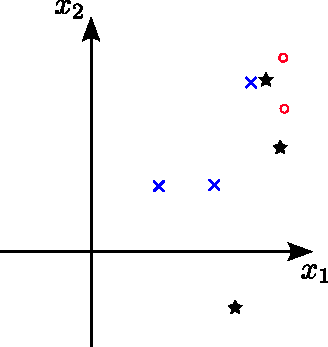
\includegraphics[width=0.34\textwidth]{img/parzen_data}}%
     \begin{subfigure}[t]{0.37\textwidth}
         \centering
         \usebox{\imagebox}% Place largest image
         \caption{Two-class data in 2D}
         \label{fig:quadratic}
     \end{subfigure}
     \hspace{2mm}
     \begin{subfigure}[t]{0.37\textwidth}
         \centering
         \raisebox{\dimexpr.5\ht\imagebox-.5\height}{% Raise smaller image into place
         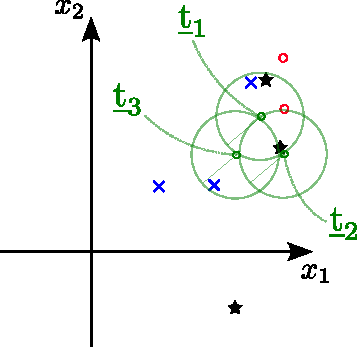
\includegraphics[width=0.99\textwidth]{img/rbf-network}
         }
         \caption{$k=3$ ``representatives''}
         \label{fig:rbf-network}
     \end{subfigure}
\end{figure}

\end{frame}

\subsection{Recap: Regression on transformed data using nonlinear basis functions}


\subsection{Nonlinear basis function}


\begin{frame}\frametitle{\subsecname}

Feature transformation $(\vec x\in \R^N)$:

\begin{equation}
\vec \phi: \vec x \mapsto \vec \phi(\vec x)
\end{equation}

\mode<article>{$\phi(\vec x)$ can transform our $N$-dim input $\vec x$ into the feature space spanned by the $k$ basis functions positioned at $\vec t_1,\ldots,\vec t_k$.
}

Assume $\{\vec t_i\}$ and corresponding kernel width $\{\sigma_i\}$ have already been determined.

Transform the feature space using \emph{radial basis functions} (Gaussian kernel functions):

\begin{align}
\phi_i(\vec x) \in 
\exp\left( -\,\frac{\lVert \vec x - \vec t_i\rVert^2_2}{2\,\sigma_{i}^2} \right), \quad i=1,\ldots,k
\end{align}

\end{frame}

\subsection{Setting for binary classification/ scalar regression}

\begin{frame}\frametitle{\subsecname}

\underline{Data}:\\

\begin{table}[h]
\begin{tabular}{rl}
transformed input & $\vec \phi^{(\alpha)} := \vec \phi(\vec x^{(\alpha)}) = \big ( 
\underbrace{1}_{\phi_{0}},
\phi_{1}(\vec x^{(\alpha)}), \ldots, \phi_{k}(\vec x^{(\alpha)}) \big)^{\top}$\\
&$\Rightarrow \vec \phi^{(\alpha)} \in \R^{k+1}$ \\[2mm]
label         & $y_{T}^{(\alpha)} \in \R$ \\
with & $\alpha = 1,\ldots,p$
\end{tabular}
\end{table}

\end{frame}

\begin{frame}\frametitle{\subsecname}

\underline{Model}:
\vspace{-5mm}
\only<1>{
	\begin{center}
		\raisebox{-3.35cm}{\includegraphics[height=5.25cm]%
			{img/section1_fig38_v2} }
		$ = \sum\limits_i \mathrm{w}_i \phi_i(\vec{x})$
	\end{center}
}
\vspace{-5mm}
\notesonly{The output is a linear neuron on the \emph{the transformed} input:}

\begin{equation}
    y(\vec \phi; \vec w) = \sum_{i=0}^{k} w_{i} \phi_{i}(\vec x) = \vec w^{\top} \vec \phi
\end{equation}

\notesonly{
Start from $i=0$ to include bias node (unlike the case with monomials where the bias was already present at $i=1$).
}
\slidesonly{Don't forget the bias!
}
Set $\vec \Phi = \left( \vec \phi^{(1)},\ldots, \vec \phi^{(\alpha)},\ldots, \vec \phi^{(p)}\right) \in \R^{k+1,p}$

quadratic cost function. \pause Reuse solution for linear regression:

\begin{equation}
\vec w^{*} = \left( \vec \Phi \, \vec \Phi^{\top}\right)^{-1} \vec \Phi \, \vec y_{\text{True}}^{\top}
\end{equation}

\question{What about using RBF-Networks for classification?}

\pause

- The quadratic cost function can still be applied to learning the parameters in an RBF-Network for solving classification problems as well but the performance is often less than when using cross-entropy loss.

\end{frame}

\subsection{Multi-dimensional RBF-Networks}

\begin{frame}\frametitle{\subsecname}

Generalizing nonlinear basis functions in linear models:

\begin{equation}
\vec y(\vec \phi(\vec x)) = 
\rmat{
y_1(\vec \phi(\vec x))\\
y_2(\vec \phi(\vec x))\\
\vdots\qquad\\
y_M(\vec \phi(\vec x))
}
= \vec W^\top \kern-.5ex \phi(\vec x)
\end{equation}

with $\vec W \in \R^{k+1,M}$

closed form solution for quadratic cost: 

\begin{equation}
\vec W^{*} =
\underbrace{
\left(\vec \Phi \, \vec \Phi^{\top} \right)^{-1}
}_{
\substack{
\text{assume}\\ \text{invertibility}}
}
\vec \Phi \, \vec Y_{\text{True}}^{\top}
\end{equation}

\question{What is $\vec Y_{\text{True}}$? What is the shape of this matrix?}

\pause

where $\vec Y_{\text{True}} := \left( \vec y_{\text{True}}^{(1)},\ldots,\vec y_{\text{True}}^{(p)}\right) \in \R^{M,p}$

\end{frame}

\begin{frame}
Remarks:

\begin{itemize}
\item RBF-Networks are universal function approximators like MLPs.
\item RBF-Networks suffer from the ``curse of dimensionality''
\item Regularization is needed:

For weight decay:
\begin{equation}
\vec W^{*} = \left( \vec \Phi \, \vec \Phi^{\top} + \lambda\,\vec I_{k+1} \,\right)^{-1} \vec \Phi \, \vec Y_{\text{True}}^{\top}
\end{equation}

\end{itemize}

\end{frame}

\subsection{RBF-Network vs. Parzen window classification}

\begin{frame}\frametitle{\subsecname}

\mode<presentation>{
\begin{equation}
\vec y_{\text{Parzen}}(\vec x) := \frac{1}{Z} \sum_{\alpha=1}^{p} \vec y_T^{(\alpha)}\, \kappa(\vec x, \vec x^{(\alpha)})
\qquad \text{(Parzen window classifier)}
\end{equation}
\begin{equation}
    \vec y_{\text{RBF-Net}}(\vec \phi; \vec w) = \sum_{i=0}^{k} w_{i} \phi_{i}(\vec x) \qquad \text{(RBF-Network)}
\end{equation}
}

\question{Which model class is a generalization of the other?}

\pause 

\question{How would you construct an RBF-Network to mimic a Parzen window classifier?}

\pause

- An RBF-Network can be constructed and parameterized to act as a Parzen window classifier by placing a ``representative'/centroid over every point $^{(\alpha)}$.





\end{frame}

\begin{frame}

\question{Can an RBF-Network solve this problem? How?}

	\begin{center}
		\raisebox{-3.35cm}{\includegraphics[height=5.25cm]%
			{img/circular} }
	\end{center}

\end{frame}

\begin{frame}

\question{Can an RBF-Network solve this problem? How many basis functions does it need?}

	\begin{center}
		\raisebox{-3.35cm}{\includegraphics[height=5.25cm]%
			{img/sdata} }
	\end{center}

\end{frame}

\begin{frame}

\question{Can an RBF-Network solve this problem using only 2 centroids?}

	\begin{center}
		\raisebox{-3.35cm}{\includegraphics[height=5.25cm]%
			{img/circular_3classes_v2} }
	\end{center}

\end{frame}

\subsection{MLPs vs. RBF-Networks}

\notesonly{cf. Haykin 5.11}

\begin{frame}

\slidesonly{\vspace{-2mm}
}
{
\slidesonly{\footnotesize}
\begin{table}[h]
\begin{tabular}{|l|l|}
\hline
\multicolumn{1}{|c|}{MLPs}                                                                          & \multicolumn{1}{c|}{RBF-Networks}                                                                                                      \\ 



\hline\pause

global approximation                                                                                &                                                                                          \begin{tabular}[c]{@{}l@{}}local approximation\\due to exponentially decaying non-linearity\end{tabular}                            \\ 
\hline\pause

\begin{tabular}[c]{@{}l@{}}+ better performance than RBF \\ with same \# of parameters\end{tabular} & \begin{tabular}[c]{@{}l@{}}- less performance than MLP \\ with same \# of parameters\end{tabular}                                      \\ 
\hline\pause

\begin{tabular}[c]{@{}l@{}}+ usually better performance\\ with larger datasets\end{tabular}         & + suitable for small datasets                                                                                                          \\ 
\hline\pause

- data hungry                                                                                       & \begin{tabular}[c]{@{}l@{}}+ faster training with \\ small \# of basis functions\end{tabular}                                          \\ 
\hline\pause

+ adapts functions to data and labels                                                               & \begin{tabular}[c]{@{}l@{}}can benefit from unlabeled data\\ (semi-supervised learning)\end{tabular}                                   \\ 
\hline\pause

\begin{tabular}[c]{@{}l@{}}common neuronal mode \\between hidden and output neurons\end{tabular}                  & \begin{tabular}[c]{@{}l@{}}The hidden layer serves a \\very different purpose\\than the output layer\end{tabular} \\ 
\hline\pause

\begin{tabular}[c]{@{}l@{}}total input of a hidden neuron\\determined via inner product\\$\vec w_i^\top x$\end{tabular}                  & \begin{tabular}[c]{@{}l@{}}total input is based on a Euclidean distance\end{tabular} \\ 
\hline\pause

\begin{tabular}[c]{@{}l@{}}\end{tabular}                  & \begin{tabular}[c]{@{}l@{}}restricted function class (many \\ basis functions needed\\ for complicated approximations)\end{tabular} \\ 
\hline\pause

\begin{tabular}[c]{@{}l@{}}\end{tabular}                             & \begin{tabular}[c]{@{}l@{}}benefits from clustered structure\\ in the data\end{tabular}                                                \\ \hline
\end{tabular}
\end{table}
}

\end{frame}

